\chapter{研究材料与研究方法}
\label{chapter:methods}

我们提出了含有非同步释放的突触模型后,先基于实验数据对模型参数进行拟合,再进行仿真实验。

\section{实验材料}
\label{section:methods:materials}

用于参数拟合的实验数据来自前人实验里快速发放神经元的突触数据,数据采集的更多细节可以参考原始实验文献\cite{Jiang2012}。

\section{分析方法}
\label{section:methods:methods}

我们先对实验数据进行预处理,得到相关的统计信息,然后进行模型的参数拟合。

\subsection{数据预处理}
\label{section:methods:data-preprocessing}

\subsubsection{估计突触电流}
实验记录到的细胞膜电流包括细胞膜的漏电流 $I_\text{leaky}(t)$ 和由于突触信号传递导致的突触电流 $I_\text{syn}(t)$ 。

细胞产生漏电流的离子通道一般是受细胞膜电位调控的,实验条件下细胞膜电位被固定,可以假设漏电流恒定不变。
通过读取突触前细胞发放前一小段时间内突触后神经元的细胞膜电流,通过计算平均值可以得到漏电流 $I_\text{leaky}$ 。
记录的电流减去漏电流 $I_\text{leaky}$ 就能得到突触电流 $I_\text{syn}(t)$ 。
对于抑制性神经元的突触,它所产生的突触电流应该为非正值,但由于噪声的存在,可能有部分时间点 $t$ 时 $I_\text{syn}(t) > 0$。
这时需要对数据进行修正,先取一个极小的电流 $\epsilon > 0$ 作为阈值,对于 $I_\text{syn}(t) > -\epsilon$ 的时间点,将 $I_\text{syn}(t)$ 修改为 $-\epsilon$。
为了不引入太大的偏差, $\epsilon$ 需要足够小。
试验中取了 $\epsilon = 0.2$ pA,相对于IPSC的大小,这是一个非常小的值。

\subsubsection{去卷积方法}
根据突触后模型式\ref{equation:synaptic-current-general}和式\ref{equation:receptor-conductance-general},假设突触后神经元细胞膜电位为常数,则 $I_\text{syn}$ 可以表示成卷积的形式
\begin{equation}
I_\text{syn}(t) = \int_{-\infty}^t e^{-\frac{t - t'}{\tau_\text{GABA}}} A q(t' - t_\text{delay}) \dd{t'}
\label{equation:synaptic-current-convolution}
\end{equation}
其中 $A = w(v - E_\text{GABA})$。
实验条件下, $v$ 是稳定的常数,$E_\text{GABA}$ 在细胞处于平衡态时也应该是一个稳定的常数,因此可以假设实验中的递质释放率 $q(t)$ 和 突触电流 $I_\text{syn}$ 有式\ref{equation:synaptic-current-convolution}中的关系。
由于 $w$ 和 $E_\text{GABA}$ 是未知常数,所以 $A$ 也是未知常数,根据 $I_\text{syn}$ 最终只能得到 $Aq(t)$。

理论上可以使用傅里叶变换来曲卷积,得到估计的释放率 $q_e(t)$。
由于
\begin{equation}
I_\text{syn} = A \cdot K * q
\label{equation:synaptic-current-convolution-theory}
\end{equation}
其中 $K(t) = \cdot e^{-\frac{t}{\tau_\text{GABA}}}$, $*$ 表示卷积。
对式\ref{equation:synaptic-current-convolution-theory}进行傅里叶变换得到
\begin{equation}
F(I_\text{syn}) = A \cdot F(K) \cdot F(q)
\label{equation:synaptic-current-fourier-transformation}
\end{equation}
$F(f)$ 表示函数 $f$ 的傅里叶变换。
因此可以得到
\begin{equation}
A \cdot F(q) = \frac{F(I_\text{syn})}{F(K)}
\label{equation:release-rate-fourier}
\end{equation}
进行逆变换则可得到
\begin{equation}
A \cdot q = F^{-1}\left( F(I_\text{syn}) / F(K) \right)
\end{equation}

但实际试验中,由于IPSC的波形中高频傅里叶分量不可忽略,进行离散傅里叶变换会造成较大的误差。
即
\begin{equation}
\left| I_\text{syn} - A \cdot K * q_e \right| \gg 0
\label{equation:deconvolution-error}
\end{equation}

另一种通用的去卷积方法(MATLAB中的deconv函数)得到的 $q_e$ 波动剧烈且有大量 $q_e(t) < 0$ 的点存在。

因此在分析数据时使用了自己提出的曲卷积方法,此方法利用了式\ref{equation:synaptic-current-convolution-theory}中 $K$ 的特点,理论上只对指数衰减型的 $K$ 适用。
虽然降低了通用性,但能够避免前两种方法的缺点。

从试验记录中预处理得到的 $I_\text{syn}$ 的时间分辨率为 $\dd{t} = 0.05$ ms。
可将时间段 $[0, T]$ 分为 $N = T/\dd{t}$ 个宽度为 $\dd{t}$ 的小区间。
在离散形式下,第 $i$ 个时间区间内的突触电流为
\begin{equation}
I_\text{syn}(i) = \sum_{j=1}^i K(i-j)q(j-\Delta)\dd{t}
\label{equation:synaptic-current-discrete-convolution} 
\end{equation}
其中当 $i \geq j$ 时,$K(i-j) = Ae^{-(i-j)\dd{t}/\tau_\text{GABA}}$,当 $i < j$ 时,$K(i-j) = 0$,$\Delta = t_\text{delay}/\dd{t}$。

首先,通过确定 GABA 递质接收器的衰减常数 $\tau_\text{GABA}$ 来确定 $K$。
使用 MATLAB 的 Curve Fitting Toolbox。
拟合的目标函数为 $\text{fittype}(@(A, t_0, \tau, leaky, t) A .* \exp(-(t-t_0)/\tau) .* (t > t_0) + leaky)$。
表示
\begin{equation}
I_\text{syn}(t) = 
\begin{cases}
A \cdot e^{-(t-t_0)/\tau_\text{GABA}} + I_\text{leaky}, & \text{若 } t > t_0 \\
I_\text{leaky}, & \text{若 } t \leq t_0
\end{cases}
\end{equation}

通过分析自发释放和单个动作电位导致的释放,得到突触的参数 $\tau_\text{GABA}$。
对于快速发放神经元到快速发放神经元的突触, $\tau_\text{GABA} \approx 2.6$ ms。
对于快速发放神经元到金字塔形神经元的突触, $\tau_\text{GABA} \approx 5$ ms (见图\ref{figure:decay-time-constant})。
这与之前文献的记录相符\cite{Bartos2002}。

\begin{figure}
\centering
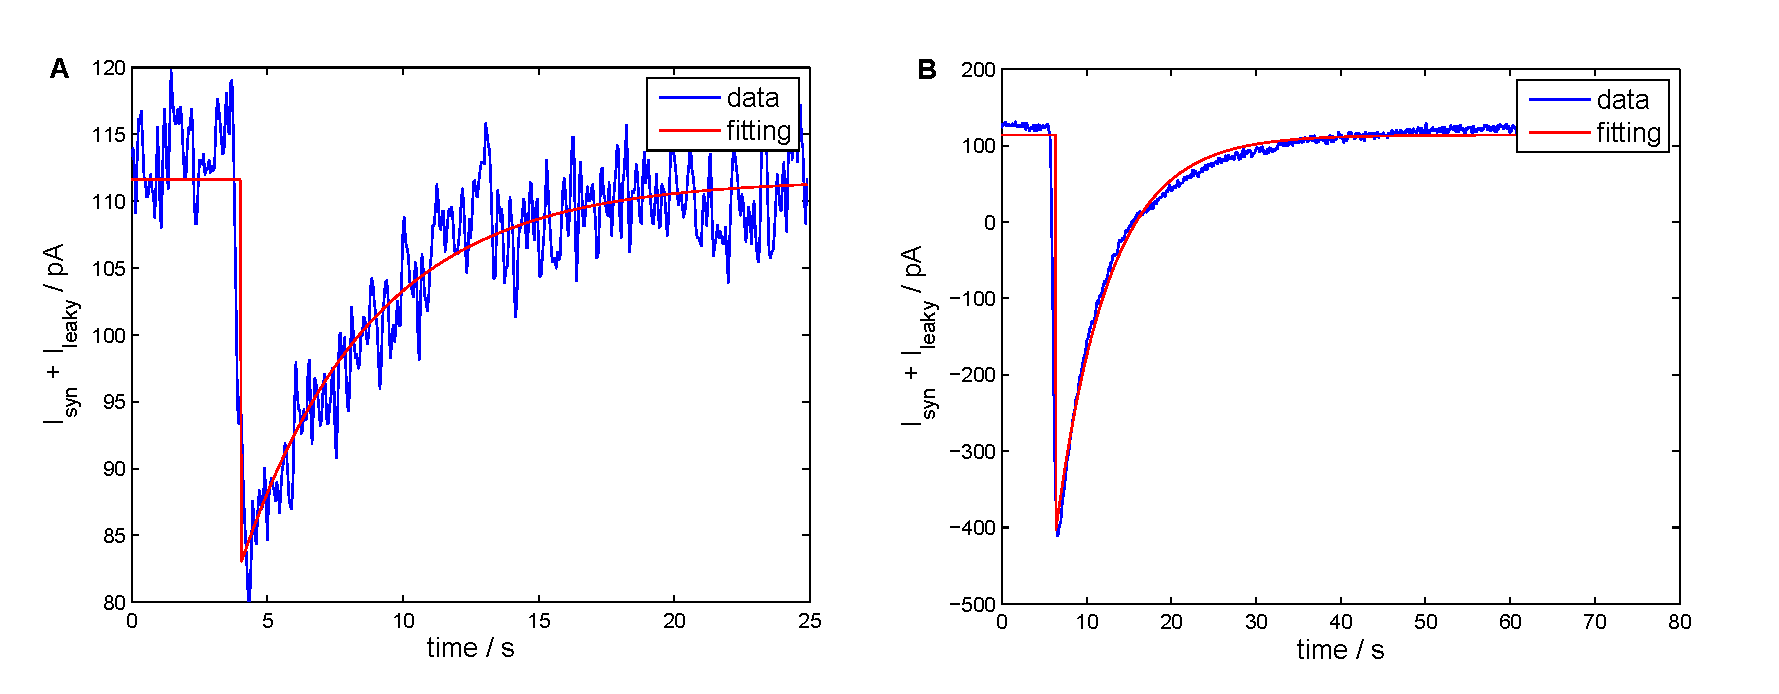
\includegraphics[scale=0.5]{fs-pc-decay-time-constant.eps}
\caption{拟合GABA递质接收器的衰减常数 $\tau_\text{GABA}$。实验数据来自癫痫病人的脑组织切片中快速发放神经元到金字塔形神经元的突触。蓝线表示实验记录的 IPSC ,红线为拟合的结果。
(A)为自发的递质释放,得到的估计值为 $\tau_\text{GABA} \approx 4.8$ ms (置信区间为 $4.39$ ms - $5.27$ ms)。
(B)为单个动作电位引发的递质释放,得到的估计值为 $\tau_\text{GABA} \approx 6.2$ ms (置信区间为 $6.06$ ms - $6.46$ ms)。}
\label{figure:decay-time-constant}
\end{figure}


得到了 $K$ 之后,使用贪心策略,一步一步递进得到 $Aq(i - \Delta)$ 对于 $i - \Delta = 1,2,\cdots,N$ 的所有值。
初始状态下 $Aq = 0$,在第 $i$ 步,假设 $q(j - \Delta)$ 在 $j = 1,2,\cdots,i-1$ 时已经得到估计值,此时我们选取 $q(i - \Delta)$ 为
\begin{equation}
\begin{split}
q(i - \Delta) &= \Argmin_{p \geq 0} \left| \sum_{j=1}^{i-1} K(i-j)q(j-\Delta)\dd{t} + Ap\dd{t} - I_\text{syn}(i) \right| \\
\text{且满足 } & \forall k \geq i, I_\text{syn}(k) \geq e^{-(k-i)\dd{t}/\tau_\text{GABA}} \cdot J(i)
\end{split}
\end{equation}
其中 $J(i) = \sum_{j=1}^{i-1} K(i-j)q(j-\Delta)\dd{t} + Ap\dd{t}$。
这样得到的估计值 $Aq_e(t - t_\text{delay})$ 满足 $A \cdot K * q_e \leq I_\text{syn}$。
约束条件 $\forall k \geq i, I_\text{syn}(k) \geq e^{-(k-i)\dd{t}/\tau_\text{GABA}} \cdot J(i)$ 保证了第 $i$ 步之后存在 $Aq \geq 0$ 的值满足$A \cdot K * q_e \leq I_\text{syn}$。

结果显示得到的 $Aq_e$ 进行卷积后与 $I_\text{syn}$ 非常接近(见图\ref{figure:deconvolution-and-latency}A-B)。
\begin{figure}
\centering
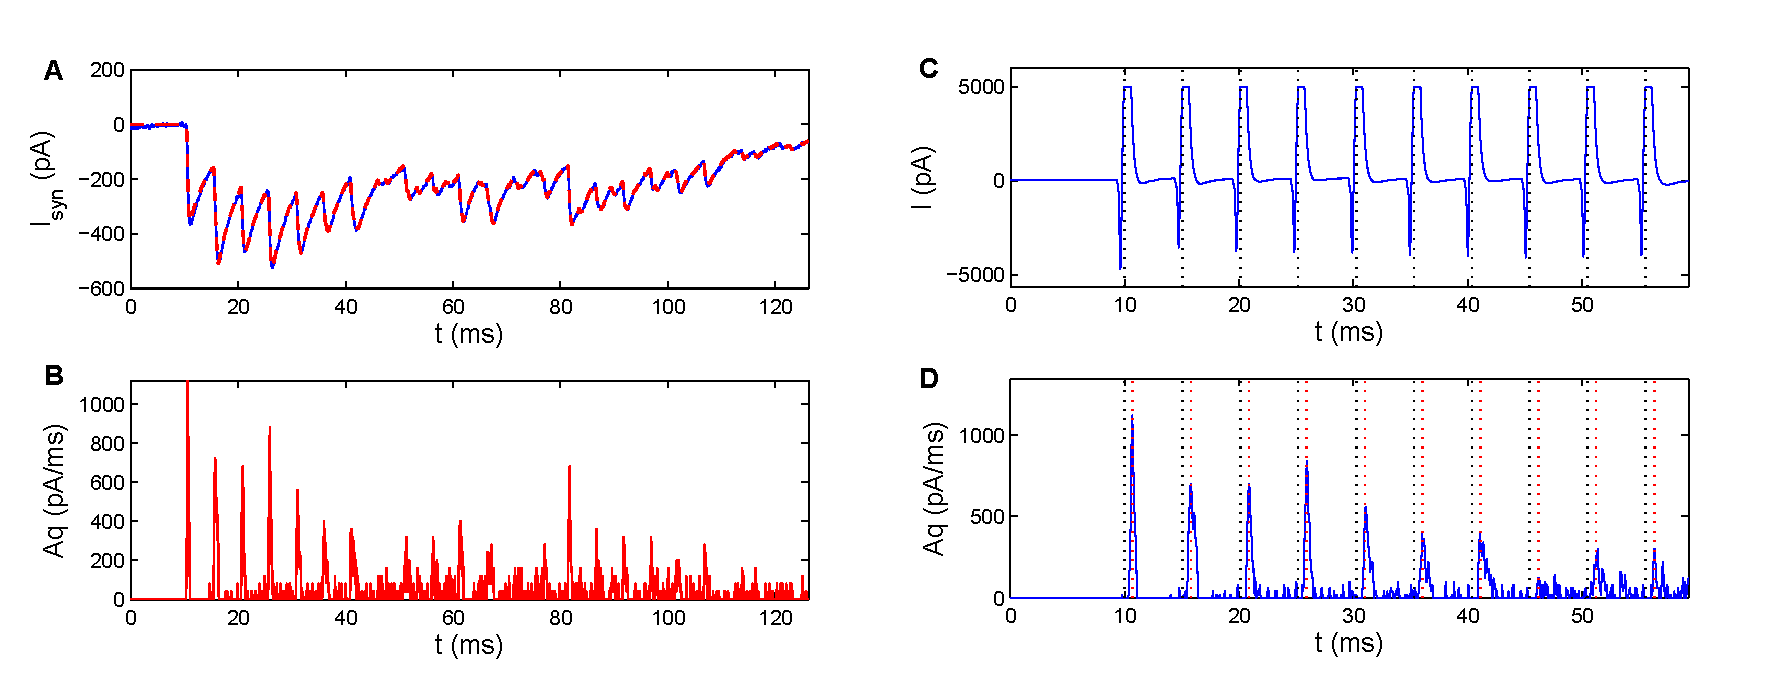
\includegraphics[scale=0.5]{fs-pc-deconvolution-and-latency.eps}
\caption{IPSC的去卷积。数据来自人类癫痫患者脑组织切片中快速发放神经元到金字塔形神经元的突触。
(A)蓝线为原始的一部分IPSC记录。红色虚线为基于 $Aq_e$ (来自B) 进行卷积后得到的结果。
两条曲线非常接近。
(B)根据实验数据分析出的IPSC(来自A)估计出的递质释放率 $\tilde{q} = Aq$。
(C-D)通过比较突触前神经元的发放时间(黑色虚线)和 $Aq(t-t_\text{delay})$ 的极高点得到 $t_\text{delay}$。
(C)突触前神经元的细胞膜电流,黑色虚线选择为神经元发放的时间。
(D)黑色虚线与 C 中时间一致,每个红色虚线比相应的黑色虚线晚 $0.75$ ms,与释放率的极高点大致重合。所以突触传递的延迟 $t_\text{delay}$ 约为 $0.75$ ms。
}
\label{figure:deconvolution-and-latency}
\end{figure}

\subsection{数据拟合}
\label{section:methods:data-fitting}
我们从实验数据中选取了 $n = 12$ 个记录得到了 $100$ Hz 频率发放动作电位时的递质释放率。
其中动作电位的发放次数分别为 $10$, $15$, $20$, 和 $25$,各有 $3$ 次重复实验。
为了便于比较,我们只选取前 $N_{sp} = 10$ 个动作电位的数据进行统计。

由于实验记录中噪声的存在,且非同步释放本身高度随机,所以这里通过将递质释放率分成多个时间区间分段统计平均释放率,并于模型进行比较,来确定模型的参数。

通过比较突触前神经元的细胞膜电流和估计出的释放率,我们观察到释放率的极高点相对于突触前神经元的发放大约总是落后 $t_\text{delay} = 0.75$ ms(见图\ref{figure:deconvolution-and-latency}C-D)。这个值就选取为式\ref{equation:receptor-conductance-general}中的突出传递延迟。

更多统计后发现,递质释放率在突触前神经元发放 $0.3$ ms 后开始急剧上升,持续约 $1.1$ ms 后急剧下降。
因此我们把时间分为两种区间。
第一种开始于突触前神经元每个动作电位后的 $0.3$ ms,持续 $1.1$ ms,这些区间记为同步释放区间 $P_\text{sr}^{(k,i)}$ ,表示第 $i$ 次试验中第 $k$ 个动作电位之后的同步释放区间。
第二种则是两个同步释放区间之间的时间段,记为非同步释放区间 $P_\text{ar}^{(k,i)}$。
神经递质在相应区间内的释放总量为
\begin{equation}
M_\text{r}^{(k,i)} = \int_{t \in P_\text{r}^{(k,i)}} Aq(t)\dd{t}
\end{equation}
其中 $\text{r} = \text{sr}, \text{ar}$。

得到了这些区间内的释放量后,我们采用概率推断的方法来估计模型参数,此方法与拟合 STP 模型用的某个方法类似\cite{Costa2013}。
这里同样假设某个特定释放区间内的递质释放量服从高斯分布。
因此我们只是用样本在多次实验记录中的均值和标准差来拟合模型。
\begin{align}
\mu_\text{r}^{(k)} &= \frac{1}{n} \sum_i M_\text{r}^{(k,i)} \\
\sigma_\text{r}^{(k)} &= \sqrt{\frac{1}{n}\sum_i\left( M_\text{r}^{(k,i)} - \mu_\text{r}^{(k)} \right)^2}
\label{equation:statistics-for-fitting}
\end{align}

根据定义的同步和非同步释放区间计算得到 $\bm{M_\text{r}}$ 之后,对于给定的参数组合 $\bm{\theta} = \{\tau_\text{sr}$,
$U_\text{sr}$, $\tau_\text{ar}$, $U_\text{ar}$, $\tau_d$, $X_F$, $x_0 \}$ 对实验观测 $\bm{M_\text{r}}$ 的似然度记为 $P\left(\bm{M_\text{r}}\left|\bm{\theta}\right.\right)$。

对于每一组参数 $\bm{\theta}$,相应的似然度为
\begin{equation}
 \log P\left(\bm{M_\text{r}}\left|\bm{\theta}\right.\right) = \sum_{r \in
    \{\text{sr}, \text{ar}\}}
  \sum_{k=1}^{N_{sp}} \left(-\frac{\big(\tilde{M}_{r}^{(k)}-\mu_{r}^{(k)}\big)^2}{2\big(\sigma_r^{(k)}\big)^2}
- \log\sqrt{2\pi}\sigma^{(k)} \right),
\label{equation:probabilistic-inference-log}
\end{equation}
其中 $\tilde{M}_\text{r}^{(k)}$ 计算模型在相应释放区间内的平均释放量。
此处取自然对数是为了防止数值计算时数值变化范围过大造成溢出。

由于式\ref{equation:ar-release}具有随机性,每一个时间区间内的 $\tilde{M}_\text{r}^{(k)}$ 需要多次计算取平均值。为了节省时间,我们将式\ref{equation:ar-release}简化为式\ref{equation:ar-release-simplified},即
\begin{equation*}
q_\text{ar}(t) = x(t) u_\text{ar}(t)\dd{t}
\end{equation*}
这样模型中就不再有随机性,一次计算就可以得到释放率的平均值。
这一改动同时使得 $x_0$ 变成了一个不起作用的参数,我们之后将用其他方法来估计 $x_0$ 的值。

我们得到了模型产生的释放率 $q'(t)$ 之后,用类似的方式计算模型的 $\tilde{M}_\text{r}^{(k)}$,此时同步释放区间 $P_\text{sr}^{(k,i)}$ 从发放时开始,持续 $1.1$ ms,,没有了延迟。
然后计算一个归一化参数 $A$,对应于 $w(v-E_\text{GABA})$,以此确保总释放量 $\sum \tilde{M}_\text{r}^{(k)}$ 与实验数据一致。

注意到递质的释放量与参数 $X_F$ 成正比 (根据式\ref{equation:sr-facilitation},式\ref{equation:ar-facilitation},式\ref{equation:total-release},和式\ref{equation:stp-depression}),即 $A \propto \frac{1}{X_F}$。这意味着如果不限定 $A$ 的值,就无法得到 $X_F$。因此不失一般性,在参数拟合过程中使用 $X_F = 1$。

通过网格式搜索来寻找使得似然度最大的参数组合。表\ref{table:parameters}中列出了搜索区间和推断出的结果。
\begin{table}
  \centering
  \begin{tabular}{llllll}
    \hline\hline
    & 参数 & 单位 & 值 & 搜索空间 & 置信区间 \\
    \hline
    & $U_\text{sr}$ & & $0.16$ & $[0.04, 0.40]$ & $[0.1550, 0.1605]$ \\
    & $\tau_\text{sr}$& ms & $1$ & $[1, 8]$ & $[0.10, 2.56]$ \\
    & $U_\text{ar}$ & & $0.020$ & $[0.008, 0.024]$ & $[0.0202, 0.0212]$ \\
    & $\tau_\text{ar}$ &ms & $8$ & $[4, 48]$ & $[8.022, 8.380]$ \\
    & $\tau_d$ &ms & $35$ & $[10, 100]$ & $[35.74, 39.04]$ \\
    & $X_F / x_0$& & $135$ & n.a. & n.a. \\
    \hline
\end{tabular}
\caption{网格式搜索寻找最大似然度参数组合的搜索区间和最终的搜索结果。此处 $\frac{X_F}{x_0}$ 是一个常数,表示在突触的活动区内最初的可以释放的囊泡数目。}
\label{table:parameters}
\end{table}

在找到了极优参数组合 $\bm{\hat{\theta}}$ 后,我们在参数组合的每一个维度,在更小的范围内用更密集的采样点来检查附近的参数。
每个维度的置信区间取似然度大于最大似然度 $90\%$ 的那些点。
表\ref{table:parameters}中有各维度的置信区间。

\begin{figure}
\centering
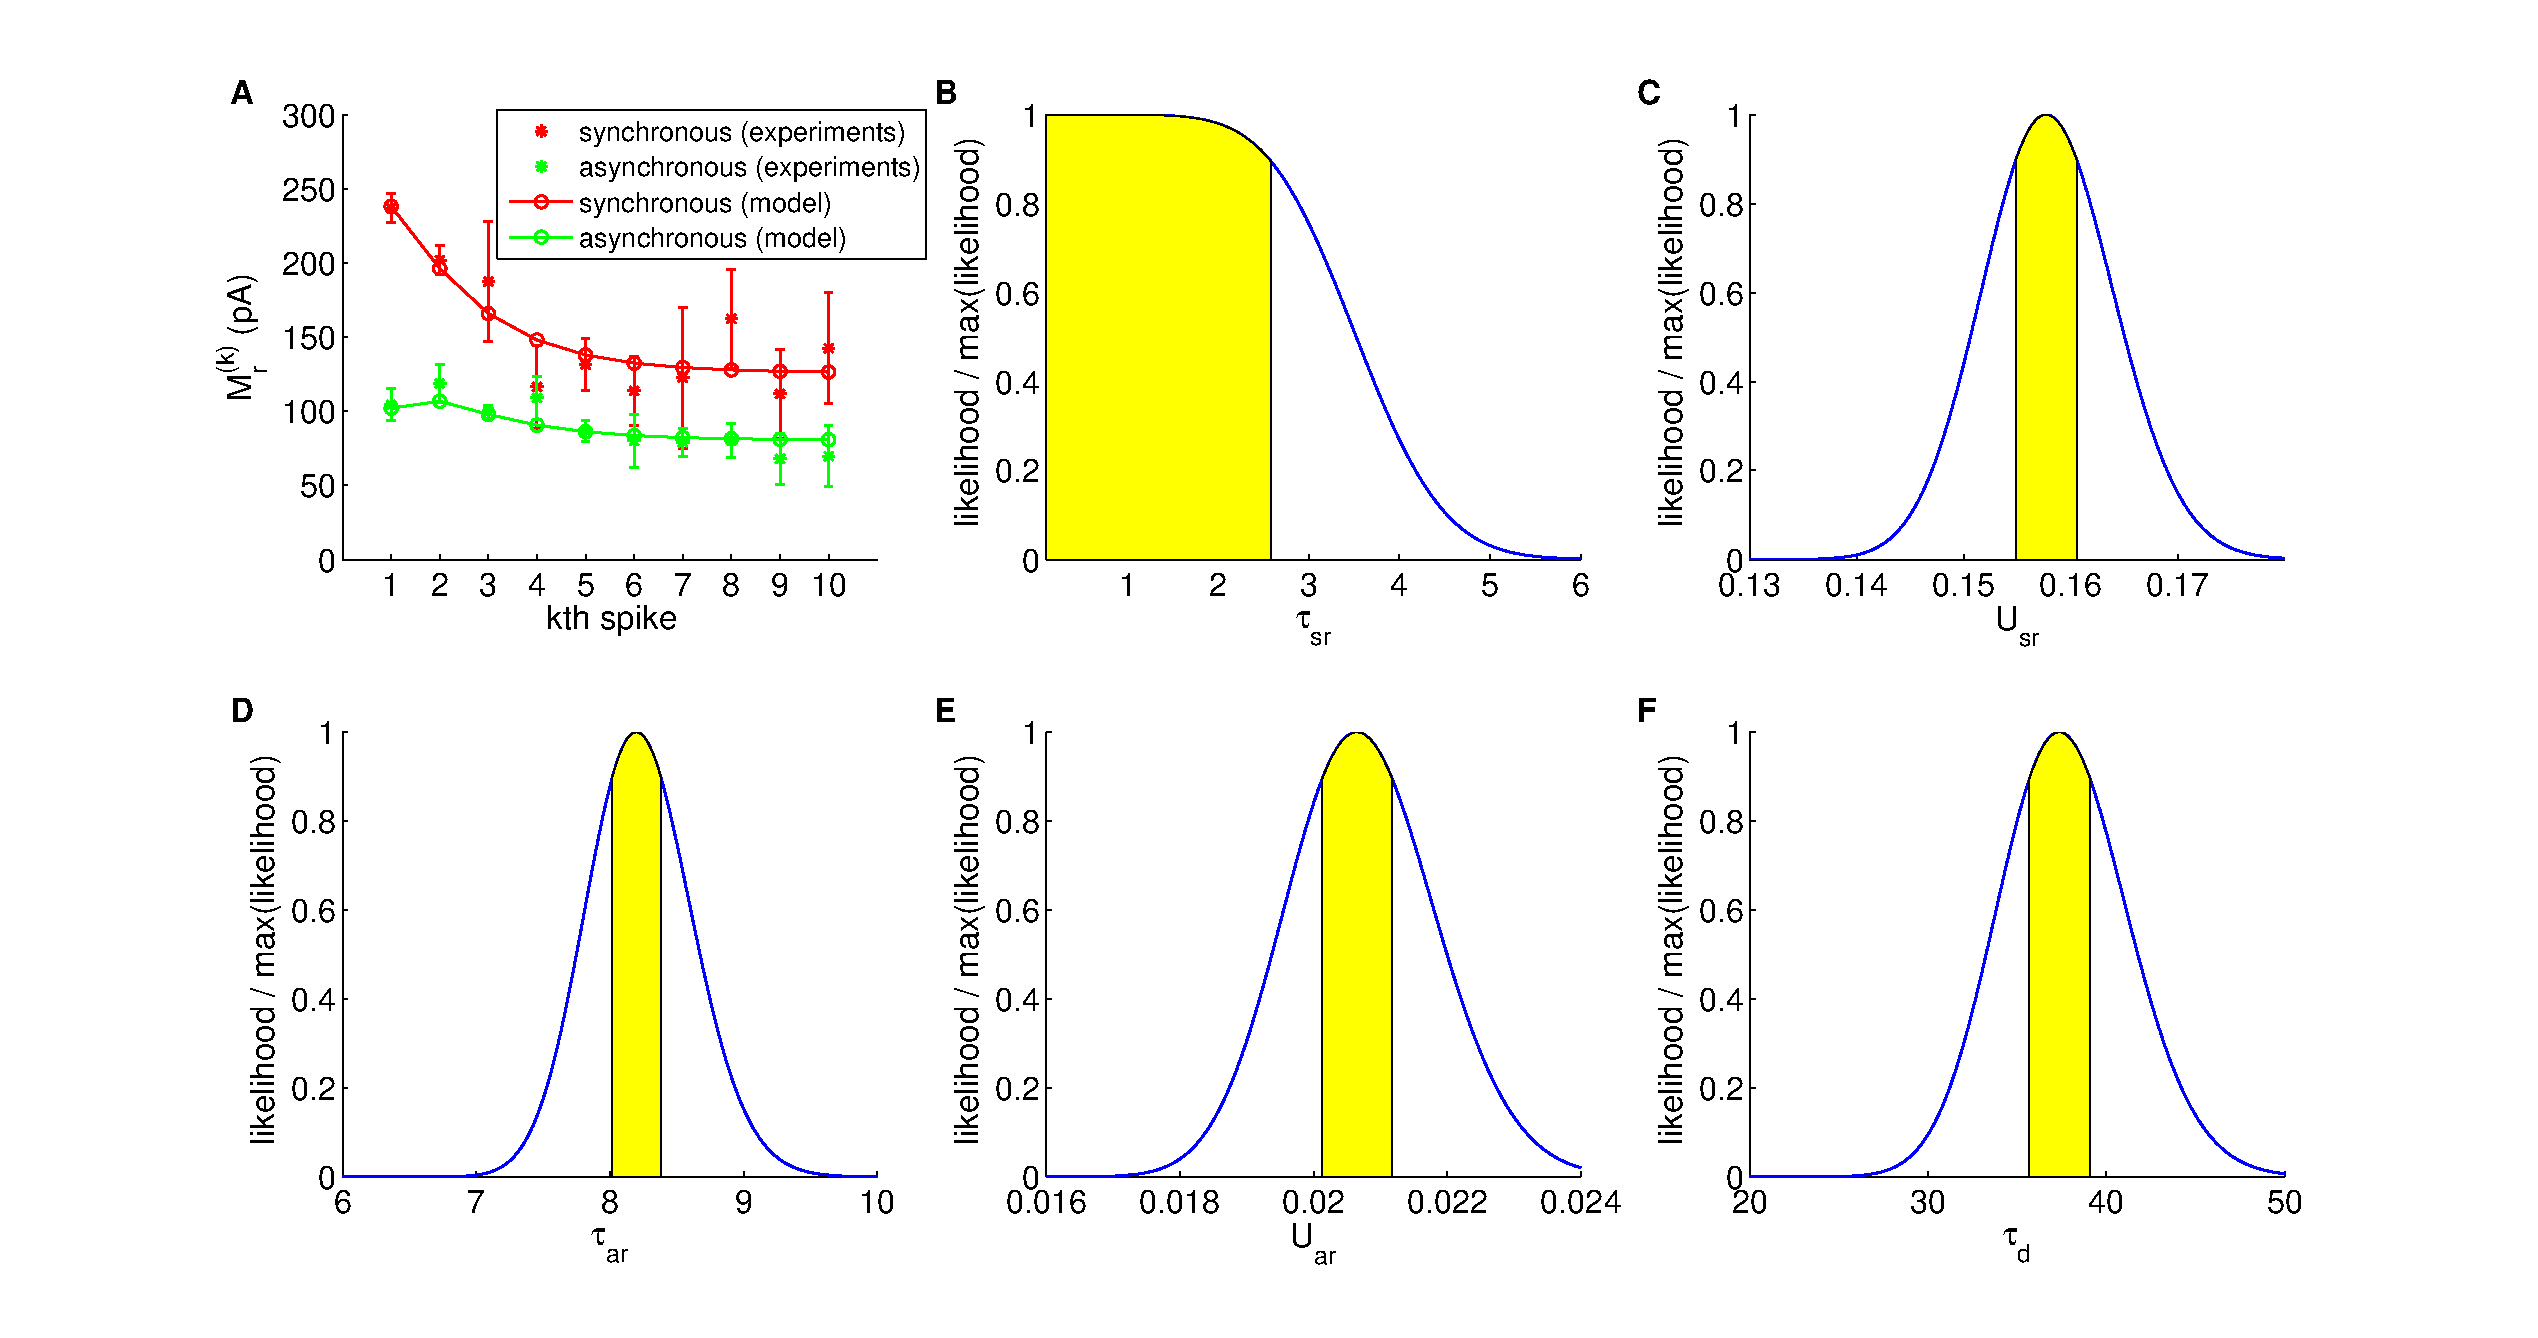
\includegraphics[scale=0.36]{fitting-results.eps}
\caption{模型参数拟合。
(A)第 $k$ 个动作电位后的平均释放量。*表示实验中统计的同步释放区间内的释放量(红色)和非同步释放区间内的释放量(蓝色)。误差棒表示标准差。实线为极优参数组合下的模型的统计数据。两者较一致。
(B-F)每个维度上在极优参数附近的置信区间。}
\label{figure:fs-pc-fitting}
\end{figure}

\subsubsection{计算囊泡释放量子}
在参数 $\tau_\text{sr}$,$U_\text{sr}$, $\tau_\text{ar}$, $U_\text{ar}$, $\tau_d$ 找到之后,我们就可以接着计算 $x_0$ 的大小。
